\chapter{Arrival Time Prediction}
\label{cha:arrival-time-prediction}

Trajectory forecasting is the process of predetermining when a bus will arrive at a particular bus stop.
The existing arrival time prediction of Östgötatrafiken AB is based purely on long-time historical data.
It provides a single timestamp when it predicts the bus to arrive at a certain bus stop.
The prediction is the most likely arrival time for the bus.

This chapter will use a methodology similar to the previous Chapter \ref{cha:GPS-variation-estimation}.
The aim is to provide a probability distribution of arrival times for the next bus stops.
This thesis project proposes a Trajectory Forecasting model based on multiple GPs.
It provides time-to-arrival probability distributions for all the remaining bus stops in the journey.
The probability distribution allows for queries such as:
\begin{itemize}
    \item \textit{What is the most likely time of arrival at bus stop $p$?}
    \item \textit{What is the probability of the bus arriving at the earliest/latest possible time?}
    \item \textit{Which stop impacts the arrival time of the bus the most?}
\end{itemize}

\section{Initial Methodology} \label{sec:initial-methodology}
The first steps of the proposed approach is similar to the steps covered in the Sections \ref{sec:stop-compression}-\ref{sec:segment-self-overlapping-journeys}.
Below is a brief description of the steps already covered, with alterations highlighted:

\begin{enumerate}
    \item \textit{Stop Model and Compression:}
    Stops during the trajectory are modelled as bus stops and red lights, i.e., common stops during a bus journey.
    GPS positions of stopped buses need to be compressed in order to support more robust GPs \cite{Tiger2018-gp-motion-pattern}.
    The result of this step is a collection of trajectories for each bus line.
    The trajectories include common stops and compressed GPS positions during stops.
    As in Section \ref{sec:stop-compression}, a \textit{Speed} threshold value of $0.1$ m/s is used for the trajectory forecasting.
    However, while stops due to traffic and red lights are compressed by removing positions occurring during a stop, they are not compressed time-wise.
    The reason behind this is to indirectly model traffic and red lights as a latent variable.
    The effects of traffic and red lights are neither explicitly modelled nor discarded.

    \item \textit{Synchronising Input Space:}
    The input space is synchronised using by training a global GP model $f_1$, given by eq. \ref{eq:gps-var-f1} in Section \ref{sec:synchronisation}.
    The model is thus
    \begin{equation*} \label{eq:gps-var-f1}
        f_1: (x, y) \longmapsto \tau,
    \end{equation*}
    and is implemented using the GPflow \cite{GPflow2017} framework.
    The GP is implemented using a Matérn covariance function (kernel) with hyperparameter $\nu =3/2$, commonly referred to as a \textit{Matern32} kernel.

    \item \textit{Segment Self-Overlapping Journeys:}
    Self-overlapping trajectories are segmented until no self-overlapping is occurring for the trajectory.
    The segmentation is required in order to avoid the problems described in Section \ref{sec:self-overlapping-trajectories}.
    Each segment will have a small model overlap, which means that neighbouring segments will share a few data points.
    This improves the robustness of the model, as it retains the desired shape close to the borders \cite{Tiger2018-gp-motion-pattern}.
    The overlap used in this thesis project is set to 5 \texttt{ObservedPositionEvent}s, which is roughly 6.5\% of an average-length segment (ca. 77 \texttt{ObservedPositionEvent}s).
\end{enumerate}

Once these three steps are executed, the approach majorly diverges compared to the approach described in Chapter \ref{cha:GPS-variation-estimation}.

\section{Segment Bus Stops}
The trajectory is segmented at bus stops, which means that the \texttt{ObservedPositionEvent}s occurring between two bus stops are segmented into one \textit{trajectory segment}.
For example, a bus line $A\rightarrow B\rightarrow C$ is segmented into two segments
\begin{enumerate}
    \item $A\rightarrow B$
    \item $B\rightarrow C$
\end{enumerate}
The positions occurring during a bus stops are already compressed by Step 1 in Section \ref{sec:initial-methodology}.
While creating the segments, the arrival time for each segment is extracted from the trajectory.
The arrival time is the date of the event where the system determines that the bus has reached the bus stop, e.g., the date when the bus reaches 
\begin{enumerate}
    \item $B$, after departing from bus stop $A$
    \item $C$, after departing from bus stop $B$
\end{enumerate}

Figure \ref{fig:segments} shows an example of the bus stop segmentation for an arbitrary trajectory.
Four sequential segments are visualised, with the relative time (in seconds) for each segment on the X-axis and the speed (m/s) of \texttt{ObservedPositionEvent}s on the Y-axis.

\begin{figure}
    \centering
    \begin{subfigure}[b]{0.475\textwidth}
        \centering
        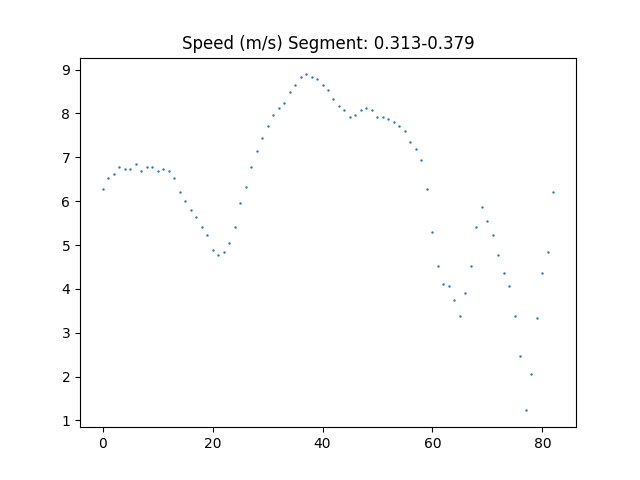
\includegraphics[width=\textwidth]{figures/segment_9}
        \caption[Segment1]%
        {{\small Segment 1}}    
        \label{fig:segment-1}
    \end{subfigure}
    \hfill
    \begin{subfigure}[b]{0.475\textwidth}  
        \centering 
        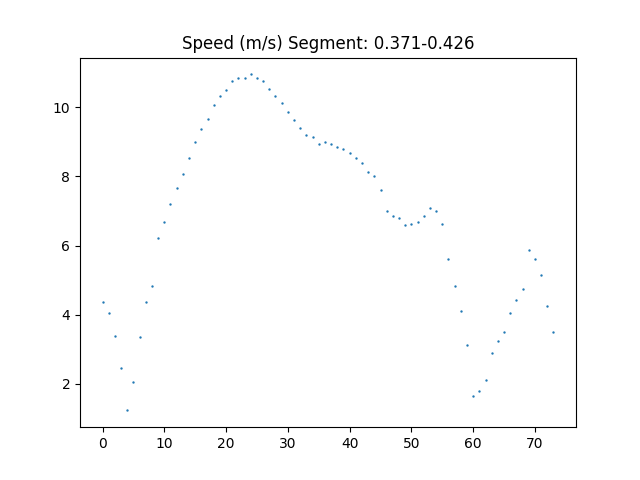
\includegraphics[width=\textwidth]{figures/segment_10}
        \caption[]%
        {{\small Segment 2}}    
        \label{fig:segment-2}
    \end{subfigure}
    \vskip\baselineskip
    \begin{subfigure}[b]{0.475\textwidth}   
        \centering 
        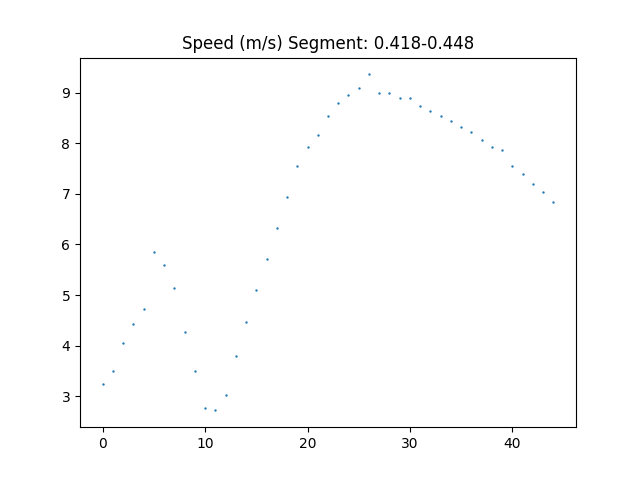
\includegraphics[width=\textwidth]{figures/segment_11}
        \caption[]%
        {{\small Segment 3}}    
        \label{fig:segment-3}
    \end{subfigure}
    \quad
    \begin{subfigure}[b]{0.475\textwidth}   
        \centering 
        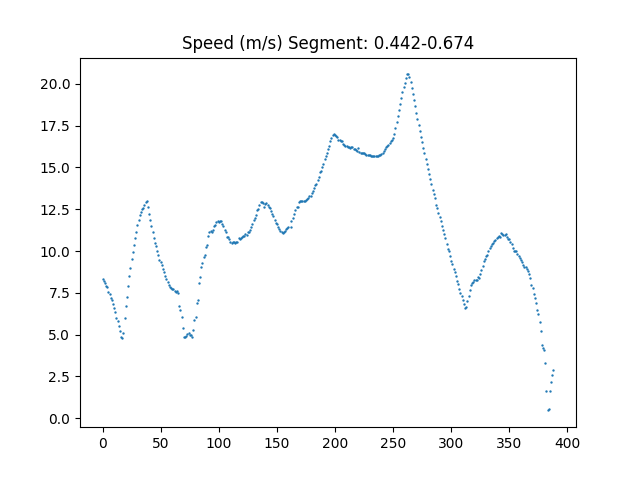
\includegraphics[width=\textwidth]{figures/segment_12}
        \caption[]%
        {{\small Segment 4}}    
        \label{fig:segment-4}
    \end{subfigure}
    \caption[ Example of trajectory segments ]
    {{\small Example of four trajectory segments with segment overlap.
    The X-axis is the relative time (in seconds) of the trajectory segment, the Y-axis is the speed of each \texttt{ObservedPositionEvent} point.}} 
    \label{fig:segments}
\end{figure}

The result of the bus stop segmentation step is a collection of segments and segment arrival times for each trajectory.

\section{Trajectory Segment Forecasting Models}
The collection of segments and arrival times are used to create features for the arrival time prediction model.
Two different GP models are created and are given by
\begin{align}
    f_A&: \tau \mapsto t_s \label{eq:f_A} \\
    f_B&: (\tau, v) \mapsto t_s \label{eq:f_B}
\end{align}
\begin{itemize}
    \item $\tau$ is the trajectory progress for the bus. $\tau$ is calculated by using GP $f_1$ from eq. \ref{eq:gps-var-f1}.
    \item $t_s$ is the predicted arrival time to the bus stop at the end of segment $s$.
    \item $v$ is the speed of the bus at $\tau$. 
\end{itemize}  

\subsection{Model Comparison $f_A$ and $f_B$}
\begin{table}
    \centering
    \caption[Arrival time prediction with the $f_B$ GP model]%
    {{\small Arrival time prediction with the $f_B$ GP model.
    The GP model predicts the arrival time for a bus driving in segment $S_0$.
    This table contains only a part of the segment $S_0$.
    Two GP models trained on segment $S_0$ are used for the prediction: $f^{(1)}_{B_0}$ and $f^{(2)}_{B_0}$.
    The right column contains the true arrival time (in seconds remaining) for the bus.}}
    \label{table:f_B-examples} 
    \begin{tabular}{ |l|l|c| } 
        \hline
        Prediction $f^{(1)}_{B_0}(S_0)$ & Prediction $f^{(2)}_{B_0}(S_0)$ & Truth $S_0$ \\ [0.5ex] 
        \hline
        48.00032032 & -176.47767445 & 48.0 \\
        46.99899913 & -207.23221327 & 47.0 \\
        46.00140604 & -233.29939699 & 46.0 \\
        44.99743229 & -263.30660917 & 45.0 \\
        44.00544805 & -291.29058078 & 44.0 \\
        42.97906806 & -326.62038041 & 43.0 \\
        42.0257244 & -339.44856005 & 42.0 \\
        40.97131472 & -358.31354569 & 41.0 \\
        40.15149734 & -374.08468248 & 40.0 \\
        39.18597533 & -377.21521534 & 39.0 \\
        38.1260134 & -385.63015598 & 38.0 \\
        36.86945791 & -383.52959391 & 37.0 \\
        35.6697429 & -378.47844965 & 36.0 \\
        35.02909338 & -382.12072838 & 35.0 \\
        33.72776512 & -408.53070845 & 34.0 \\
        33.26752095 & -410.33279089 & 33.0 \\
        31.99396506 & -441.67817682 & 32.0 \\ 
        \hline
    \end{tabular}
\end{table}

\begin{table}
    \centering
    \caption[Arrival time prediction with the $f_A$ GP model]%
    {{\small Arrival time prediction with the $f_A$ GP model.
    The GP model predicts the arrival time for a bus driving in segment $S_0$.
    This table contains the full trajectory segment $S_0$.
    Two GP models trained on segment $S_0$ are used for the prediction: $f^{(1)}_{A_0}$ and $f^{(2)}_{A_0}$.
    The right column contains the true arrival time (in seconds remaining) for the bus.}}
    \label{table:f_A-examples} 
    \begin{tabular}{ |l|l|c| } 
        \hline
        Prediction $f^{(1)}_{A_0}(S_0)$ & Prediction $f^{(2)}_{A_0}(S_0)$ & Truth $S_0$ \\ [0.5ex] 
        \hline
        27.95503975 & 65.03012452 & 48.0 \\
        27.37264309 & 65.60988244 & 47.0 \\
        26.79024643 & 66.27802379 & 46.0 \\
        26.20784977 & 66.57825337 & 45.0 \\
        25.6254531 & 66.56967009 & 44.0 \\
        25.04305644 & 66.45871024 & 43.0 \\
        24.46065978 & 66.43164454 & 42.0 \\
        23.87826312 & 66.55277654 & 41.0 \\
        23.29586646 & 66.51186703 & 40.0 \\
        22.7134698 & 64.80122062 & 39.0 \\
        22.13107314 & 60.54143875 & 38.0 \\
        21.54867647 & 56.10481638 & 37.0 \\
        20.96627981 & 52.76073634 & 36.0 \\
        20.38388315 & 50.551963 & 35.0 \\
        19.80148649 & 49.37658565 & 34.0 \\
        19.21908983 & 48.68000806 & 33.0 \\
        18.63669317 & 47.65352869 & 32.0 \\
        18.05429651 & 46.02520827 & 31.0 \\
        17.47189984 & 44.1262408 & 30.0 \\
        16.88950318 & 42.15228012 & 29.0 \\
        16.30710652 & 40.15343929 & 28.0 \\
        15.72470986 & 38.24670063 & 27.0 \\
        15.1423132 & 36.48232127 & 26.0 \\
        14.55991654 & 34.88608213 & 25.0 \\
        13.97751987 & 33.27055723 & 24.0 \\
        13.39512321 & 31.60546199 & 23.0 \\
        12.81272655 & 29.9831286 & 22.0 \\
        12.23032989 & 28.31336581 & 21.0 \\
        11.64793323 & 27.17332347 & 20.0 \\
        11.06553657 & 25.93364806 & 19.0 \\
        10.48313991 & 24.84461193 & 18.0 \\
        9.90074324 & 24.03633668 & 17.0 \\
        9.31834658 & 23.3454507 & 16.0 \\
        8.73594992 & 22.37728688 & 15.0 \\
        8.15355326 & 21.41980069 & 14.0 \\
        7.5711566 & 20.52921774 & 13.0 \\
        6.98875994 & 19.5353604 & 12.0 \\
        6.40636328 & 18.51786328 & 11.0 \\
        5.82396661 & 17.51855416 & 10.0 \\
        5.24156995 & 16.5171758 & 9.0 \\
        4.65917329 & 15.45255104 & 8.0 \\
        4.07677663 & 14.2718466 & 7.0 \\
        3.49437997 & 13.101716 & 6.0 \\
        2.91198331 & 12.2061083 & 5.0 \\
        2.32958665 & 11.09441227 & 4.0 \\
        1.74718998 & 9.68280617 & 3.0 \\
        1.16479332 & 8.31569843 & 2.0 \\
        0.58239666 & 6.04183395 & 1.0 \\
        0. & 1.62973611 & 0.0 \\
        \hline
    \end{tabular}
\end{table}

A comparison between GP models $f_A$ and $f_B$ is executed in order to find the best model for arrival time prediction.
In the comparison, both GP models use a Matérn kernel with $\nu =3/2$.

Table \ref{table:f_B-examples} shows the evaluation results of GP model $f_B$.
GP model $f_B$ is used to predict the arrival time for a particular bus driving in segment $S_0$.
GP model $f^{(1)}_{B_0}$ is trained with the same data produced by the particular bus the GP models are evaluated with.
GP model $f^{(2)}_{B_0}$ is trained on data produced by another bus.
The results from the GP model $f^{(0)}_{B_0}$ does not come with any surprises, as the model is trained on the same data used to evaluate it.
However, GP model $f^{(2)}_{B_0}$ performs extremely poorly on unseen data; which is an indication that the model does not generalise well.

Table \ref{table:f_A-examples} show the evaluation results of GP model $f_A$.
The same approach is used in the evaluation:
\begin{itemize}
    \item Both models are evaluated on the same data
    \item GP model $f^{(1)}_{A_0}$ is trained on the same data used for the evaluation.
    \item GP model $f^{(2)}_{A_0}$ is trained on different data, but for the same segment $S_0$.
    \item The right column contains the true arrival times for the evaluation data.
\end{itemize}

The evaluation resulted in heavier focus on the $f_A$ GP model.
Different kernels are tested and evaluated for the $f_A$, together with varying the hyperparameters.
The follow kernels are tested:
\begin{enumerate}
    \item Linear 
    \item White
    \item RBF
    \item RBF+Linear
    \item Matern32
\end{enumerate}
The different $f_A$ models are compared by calculating the following two metrics for each model:
\begin{enumerate}
    \item Root Mean Square Error (RMSE)
    \item Mean Absolute Error (MAE)
\end{enumerate}
The evaluation is similar to the evaluation between GP models $f_B$ and $f_A$.

The metric scores and the visual representation of the different GPs are taken into consider when choosing the best, appropriate model.
The best setting is used for the remainder of the thesis project.
GPflow also supports a wide range of optimisation algorithms.
This thesis project uses the standard L-BFGS-B algorithm.

\begin{table}
    \centering
    \caption[Metric scores for $f_A$ GP models]%
    {{\small Metric scores for $f_A$ GP models.
    The GP models predict the arrival time for a bus driving in segment $S_0$.
    The metrics are calculated by comparing the predicted arrival time to the true arrival time. 
    Two GP models are trained for each choice of kernel. 
    The model $f^{(1)}_{A_0}$ is trained on the same data as it is evaluated by.
    Model $f^{(2)}_{A_0}$ is evaluated on the same data as $f^{(1)}_{A_0}$, but is trained on different data.}}
    \label{table:metric-scores} 
    \begin{tabular}{ |c|r|r|r|r| } 
        \hline
        Kernel & RMSE $f^{(1)}_{A_0}$ & RMSE $f^{(2)}_{A_0}$ & MAE $f^{(1)}_{A_0}$ & MAE $f^{(2)}_{A_0}$ \\ [0.5ex] 
        \hline
        Linear & 24.85 & 25.26 & 20.56 & 21.49 \\
        White & 26.80 & 26.80 & 22.38 & 22.38 \\
        RBF & \textbf{1.56} & \textbf{13.53} & \textbf{0.84} & \textbf{11.69} \\
        RBF+Linear & \textbf{1.56} & 13.60 & \textbf{0.84} & 11.84 \\
        Matern32 & 11.19 & 13.56 & 9.34 & 11.75 \\
        \hline
    \end{tabular}
\end{table}

\begin{figure}
    \centering
    \begin{subfigure}[b]{0.475\textwidth}
        \centering
        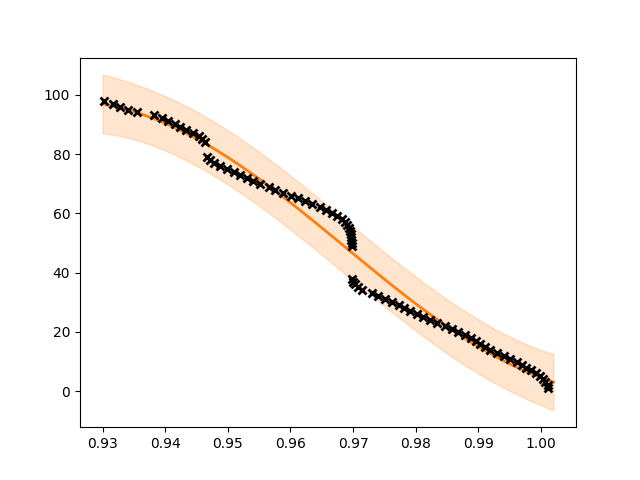
\includegraphics[width=\textwidth]{figures/forecasting/gp_3_18_rbf}
        \caption[]%
        {{\small Model of trajectory 3, segment 18,using the RBF kernel.}}    
        \label{fig:3-18-rbf}
    \end{subfigure}
    \hfill
    \begin{subfigure}[b]{0.475\textwidth}  
        \centering 
        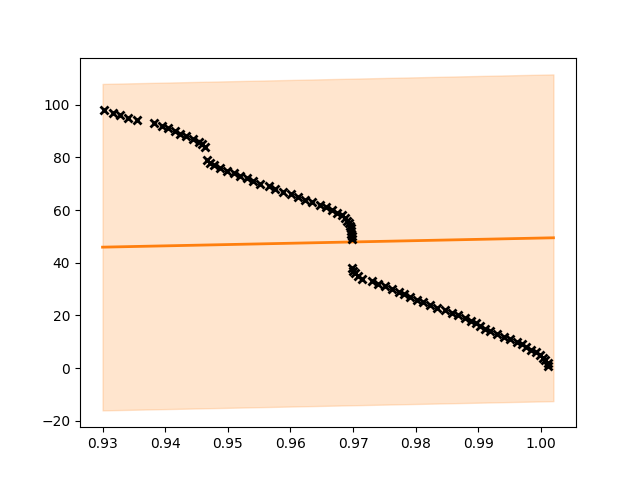
\includegraphics[width=\textwidth]{figures/forecasting/gp_3_18_rbf_linear}
        \caption[]%
        {{\small Model of trajectory 3, segment 18, using the RBF+Linear kernel.}}    
        \label{fig:3-18-rbf-linear}
    \end{subfigure}
    \vskip\baselineskip
    \begin{subfigure}[b]{0.475\textwidth}   
        \centering
        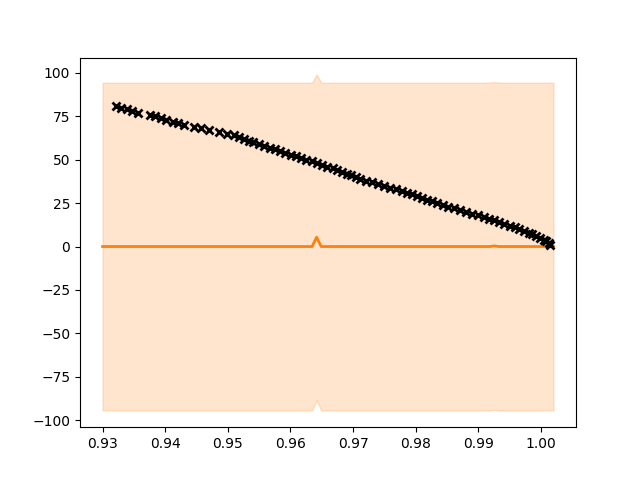
\includegraphics[width=\textwidth]{figures/forecasting/gp_5_18_rbf}
        \caption[]%
        {{\small Model of trajectory 5, segment 18, using the RBF kernel.}}    
        \label{fig:5-18-rbf}
    \end{subfigure}
    \quad
    \begin{subfigure}[b]{0.475\textwidth}   
        \centering 
        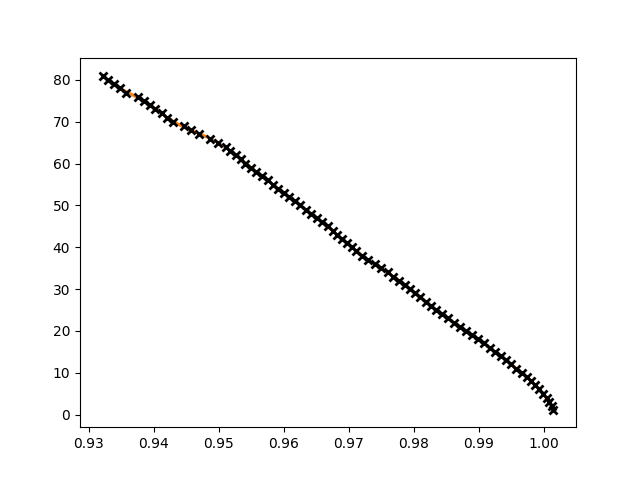
\includegraphics[width=\textwidth]{figures/forecasting/gp_5_18_rbf_linear}
        \caption[]%
        {{\small Model of trajectory 5, segment 18, using the RBF+Linear kernel.}}    
        \label{fig:5-18-rbf-linear}
    \end{subfigure}
    \caption[ Visualisation of $f_A$ models with different kernels ]
    {{\small Visualisation of $f_A$ models with different kernels.
    Each figure contains the predictive mean and variance of the model, alongside the training data points.  
    The X-axis is the $\tau$ values of the trajectory segment and the Y-axis is the arrival time to the end of the segment, in seconds.}} 
    \label{fig:5-18-3-18-models}
\end{figure}

\begin{figure}[t!]
    \centering
    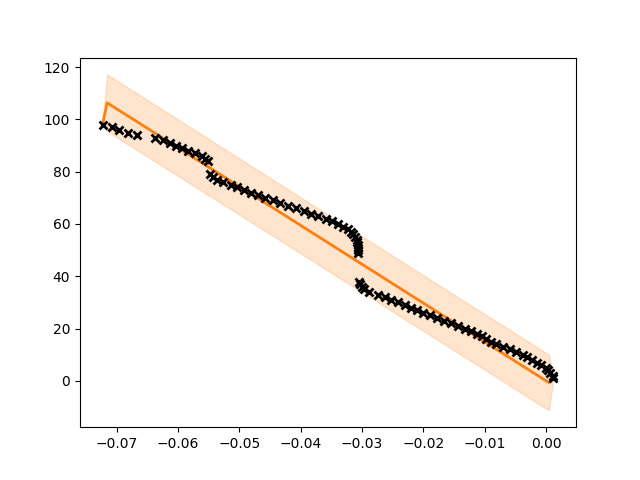
\includegraphics[width=0.475\textwidth]{figures/forecasting/gp_3_18_rbf_linear_log}
    \caption[RBF+Linear kernel with logarithmised input.]%
    {{\small RBF+Linear kernel with logarithmised input. 
    The model is trained on data from trajectory 3, segment 18.
    }}
    \label{fig:3-18-log}
\end{figure}

\begin{figure}[t!]
    \centering
    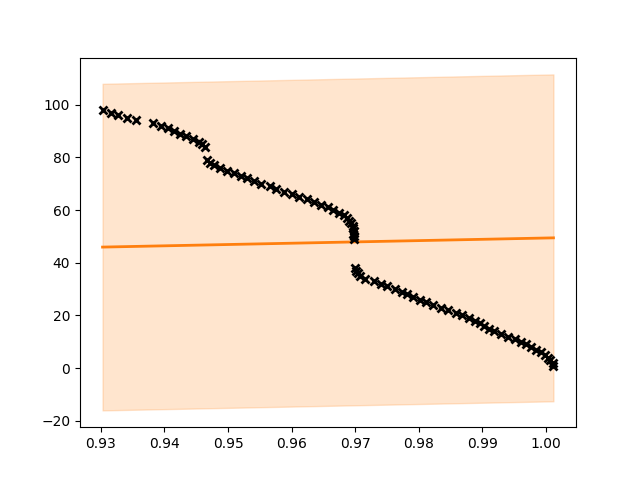
\includegraphics[width=0.475\textwidth]{figures/forecasting/gp_3_18_linear}
    \caption[Linear kernel component of the RBF+Linear model.]%
    {{\small Linear kernel component of the RBF+Linear model. 
    The model is trained on data from trajectory 3, segment 18.
    }}
    \label{fig:3-18-linear}
\end{figure}

\subsection{Model Evaluation $f_A$}
The results of the $f_A$ GP model evaluation are presented in Table \ref{table:metric-scores}.
The RBF kernel and the combined RBF+Linear kernel achieved the lowest scores.
In the general case, the RBF kernel and the RBF+Linear kernel performed equally well.
However, in some segments the different choice of kernels greatly affected the robustness of the GP model.
Figure \ref{fig:5-18-3-18-models} shows a segment for two different trajectories, were either only the RBF kernel performs well or only the RBF+Linear kernel.
While the two kernels work equally well in the general case, there are segments were neither work, depending on the trajectory.
Manual analysis of the different segments show that most segments follow a linear trend with occasional curvature.
This suggests that a RBF+Linear kernel could be more suitable in the general case.
While GPflow optimises the hyperparameters of the model, it seems like the models occasionally get stuck in a local minima, as shown in Figure \ref{fig:3-18-rbf-linear} and \ref{fig:5-18-rbf}.

Figure \ref{fig:3-18-log} shows how the model in \ref{fig:3-18-rbf-linear} performs better if the natural logarithm is applied to the input data.
The improved performance indicates that the RBF+Linear model performs better if the input values are closer, or around zero.
In Figure \ref{fig:3-18-linear}, only the Linear kernel component from the RBF+Linear model shown in Figure \ref{fig:3-18-rbf-linear} is visualised.
The figure indicates that the Linear kernel component takes over the combined kernel.
In order to try and resolve the problems, the initial hyperparameters of the RBF+Linear model are varied manually, until a stable model is acquired.

Figure \ref{fig:good-kernel-results} shows the RBF+Linear model with the following initial hyperparameters:
\begin{enumerate}
    \item $l_{RBF}=0.1$, where $l_{RBF}$ is the length-scale of the RBF kernel in the combined RBF+Linear model.
    \item $\sigma_{Linear}^2=500$, where $\sigma_{Linear}^2$ is a prior on the variance of the Linear kernel in the combined RBF+Linear model.
\end{enumerate}

\begin{figure}
    \centering
    \begin{subfigure}[b]{0.475\textwidth}
        \centering
        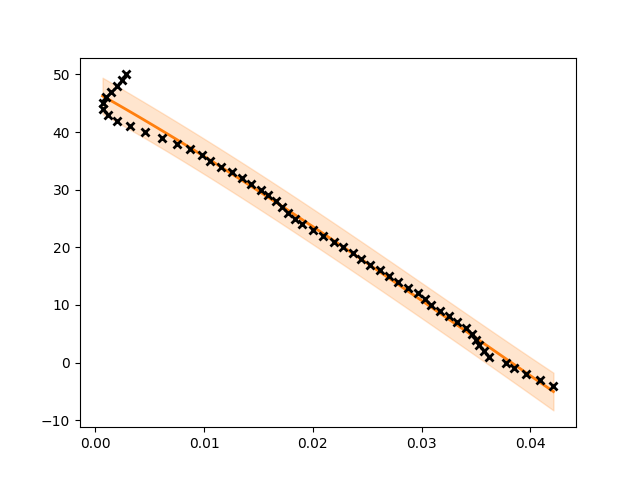
\includegraphics[width=\textwidth]{figures/forecasting/gp_2_0_rbf_linear}
        \caption[]%
        {{\small Model of trajectory 2, segment 0, using the RBF+Linear kernel.}}    
        \label{fig:2-0-rbf-linear}
    \end{subfigure}
    \hfill
    \begin{subfigure}[b]{0.475\textwidth}  
        \centering 
        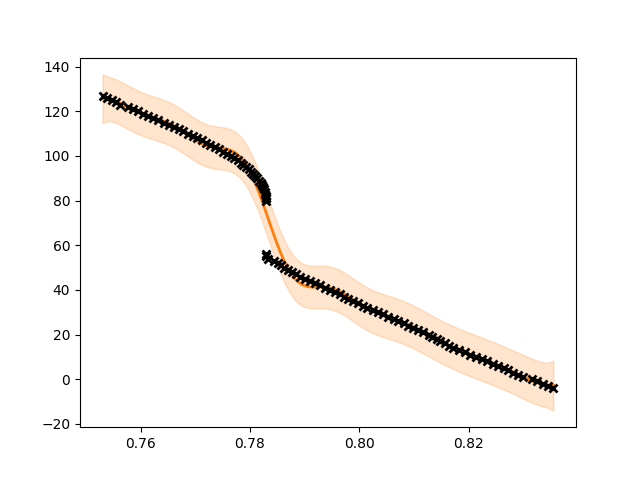
\includegraphics[width=\textwidth]{figures/forecasting/gp_4_15_rbf_linear}
        \caption[]%
        {{\small Model of trajectory 4, segment 15, using the RBF+Linear kernel.}}    
        \label{fig:4-15-rbf-linear}
    \end{subfigure}
    \vskip\baselineskip
    \begin{subfigure}[b]{0.475\textwidth}   
        \centering
        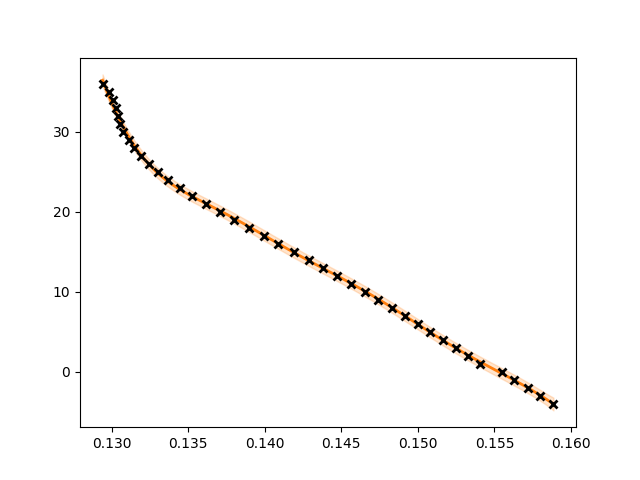
\includegraphics[width=\textwidth]{figures/forecasting/gp_16_4_rbf_linear}
        \caption[]%
        {{\small Model of trajectory 16, segment 4, using the RBF+Linear kernel.}}    
        \label{fig:16-4-rbf-linear}
    \end{subfigure}
    \quad
    \begin{subfigure}[b]{0.475\textwidth}   
        \centering 
        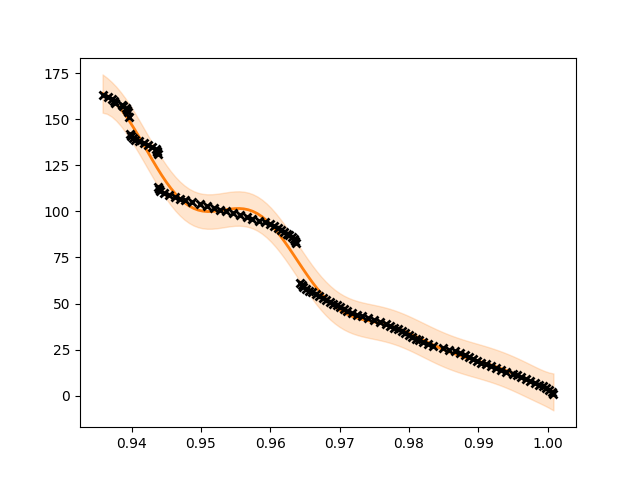
\includegraphics[width=\textwidth]{figures/forecasting/gp_26_18_rbf_linear}
        \caption[]%
        {{\small Model of trajectory 26, segment 18, using the RBF+Linear kernel.}}    
        \label{fig:26-18-rbf-linear}
    \end{subfigure}
    \caption[ Visualisation of arbitrary segments with the RBF+Linear kernel ]
    {{\small Visualisation of segments with the RBF+Linear kernel.
    Each figure contains the predictive mean and variance of the model, alongside the training data points.  
    The X-axis is the $\tau$ values of the trajectory segment and the Y-axis is the arrival time to the end of the segment, in seconds.}} 
    \label{fig:good-kernel-results}
\end{figure}


\section{Discussion}

\subsection{Kernels}
Olika kernels (modeller) för samma segment.
RBF vs RBF+Linear vs Linear

Log eller inte?

Hyperparameter initalisation.
Optimisation?

700+ models, how to initialise hyperparameters so that all work well?

$f_B$ vs $f_A$, olika kernels för olika dimensioner? Hastighet som feature?
\subsection{Common Stops}
In this thesis project only bus stops were regarded as a common stop, due to time limitations.
The approaches available were:
\begin{enumerate}
    \item \textit{Bus Stops:} 
    This is the approach used in the thesis project.
    Only bus stops were considered as common stops, as this was the simplest approach possible (beyond no segmentation at all).
    The approach would result in a probability distribution of arrival time predictions for the next bus stop.
    Red lights would be a latent variable not being modelled by the approach, which would have an impact on the probability distribution.
    \item \textit{Bus Stops and Red Lights:}
    Modelling common stops using both bus stops and red lights would probably be the optimal approach.
    Red lights are static phenomenons which either causes a change to the expected arrival time (if red light) or not (green light).
    However, deciding whether or not a stop occurred due to red lights or traffic is not trivial with the data available in the dataset.
    Stops in all trajectories for the same bus line could be compared and a common ground could be established, but what would the comparison be?
    For example, if the same stop occurs in 90\% of all trajectories and it is not a bus stop, then it is most likely a red light\todo{Hur ofta händer det här?}.
    However, traffic would still be a latent variable not modelled by the approach.
    \item \textit{All Stops:}
    This extreme approach would model all stops in each trajectory as a common stop.
    The approach would create a larger number of segments compared to the previous, more restrictive, approaches.
    A trajectory suffering from heavy traffic would create multiple segments over a potentially short distance.
    The complexity of the model would thus explode as the number of segments grow.
    However, with a large dataset this approach could be effective to also model the effects of traffic.
\end{enumerate} 

\subsection{Poor Bus Stop Detection}
Resecentrum, stannar i 3 minuter => obalans i target.

\section{Future Work}
